% %% %%%%%%%%%%%%%%%%%%%%%%%%%%%%%%%%%%%%%%%%%%%%%%%%%%%%%%%%%%
% intro-iic.tex
%
% Author:  Mauricio Matamoros
% License: MIT
%
% %% %%%%%%%%%%%%%%%%%%%%%%%%%%%%%%%%%%%%%%%%%%%%%%%%%%%%%%%%%%

%!TEX root = ../practica.tex
%!TEX root = ../references.bib

\subsection{Bus 1-Wire}%
\label{sec:intro-1wire}

\begin{wrapfigure}{r}{0.3\columnwidth}
	\centering
	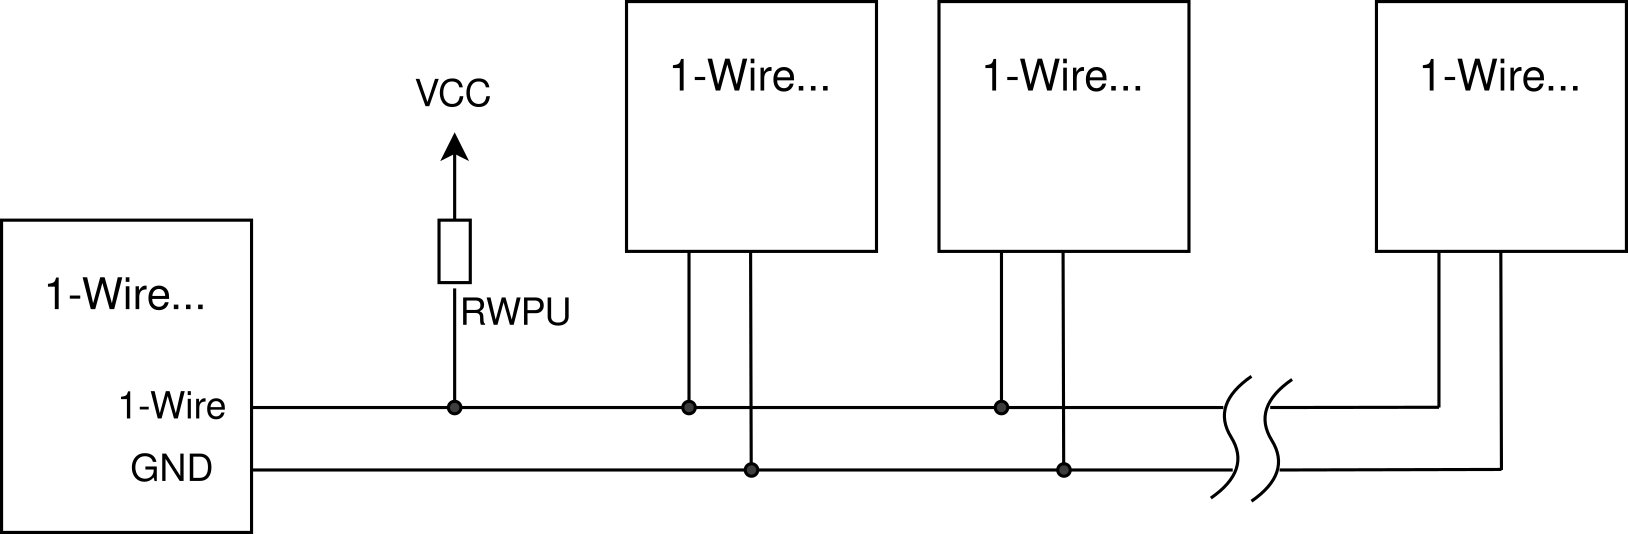
\includegraphics[width=0.3\columnwidth]{img/1-Wire.png}
	\caption{Bus 1-Wire con esclavos parásitos}%
	\label{fig:1wire-bus}
\end{wrapfigure}
1-Wire es un protocolo serial inventado por Dallas Semiconductor y diseñado para conectar dispositivos de muy baja velocidad mediante una interfaz de un sólo hilo (\Cref{fig:iic-bus}) para transmisión datos.
El bus 1-Wire es popular en meteorología (mediciones de temperatura, humedad y presión) debido a su facilidad de uso, fácil configuración y largo alcance (hasta 500 mestros)~\Citep{1WireWeb,Macekova20121}.

La transferencia de datos es serial asíncrona y transmite paquetes de 8 bits con velocidades de hasta 16.3 kbit/s y un voltaje variable entre 2.8V y 5.25V.
El dispositivo maestro, llamado MicroLAN, negocia la velocidad con los dispositivos esclavos y coordina la transmisión de datos.
Cada dispositivo esclavo es identificado mediante un paquete de 64 bits único y definido por el fabricante, donde los 8 bits más significativos especifican la familia del producto, es decir su tipo y función.
Además, la baja velocidad de operación del bus permite que el bus opere en modo \emph{parásito} con tan sólo dos hilos: datos y tierra. Esto se logra mediante la inclusión de un capacitor de 800pF que almacena energía cuando el bus de datos está activo~\Citep{1WireWeb,Macekova20121}.

Al ser un sensor completamente digital con un protocolo de transmisión de datos predefinido la lectura de datos del bus 1-Wire requiere de un controlador, mismo que viene integrado en la Raspberry Pi.
Una vez habilitado dicho controlador, éste enumerará todos los dispositivos conectados al bus 1-Wire, mismos que serán visibles bajo \texttt{/sys/bus/w1/devices}.
